Il seguente codice MatLab contiene la chiamata rispettivamente delle funzioni implementate negli esercizi precedente (\textit{es.1 y = lagrange(xi, fi, x)}, \textit{es.2 y = newton(xi, fi, x)} e \textit{es.3 y = hermite(xi, fi, f1i, x)}) con i seguenti valori di \textit{Input} :\\\ 
	\[
		f_i = sin(x) \quad [0,2\pi] \quad f'_i = cos(x)
	\]
	\[
		x_i = i\pi
		\quad
		i = 0,1,2
	\]
	\lstinputlisting[language=Matlab]{Cap_4/Es_4/Es_4.m}
Mostriamo nei seguenti plot l'approssimazione della funzione $sin(x)$ tramite l'utilizzo delle funzioni di interpolazione, precedentemente elencate:\\\
	\begin{figure}[H]
		\label{Cap4_Es_4}
			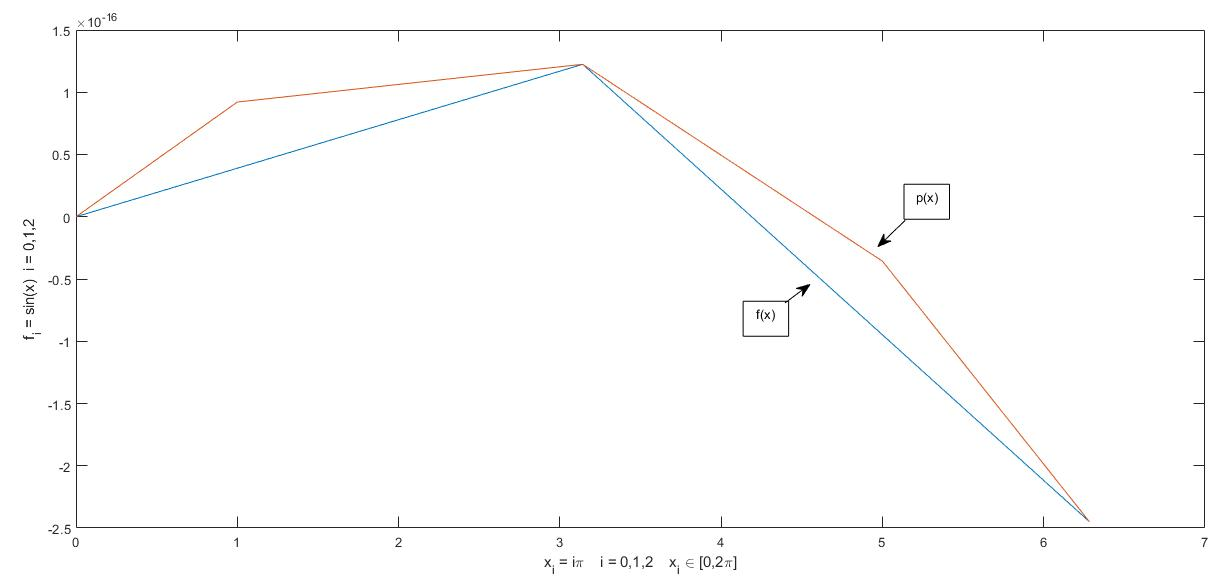
\includegraphics[left, width=150px]{Plot/Cap_4_Es_4_Lagrange_Newton}
			\caption*{Lagrange e Newton}
	\end{figure}
	\begin{figure}[H]
		\label{Cap4_Es_4}
			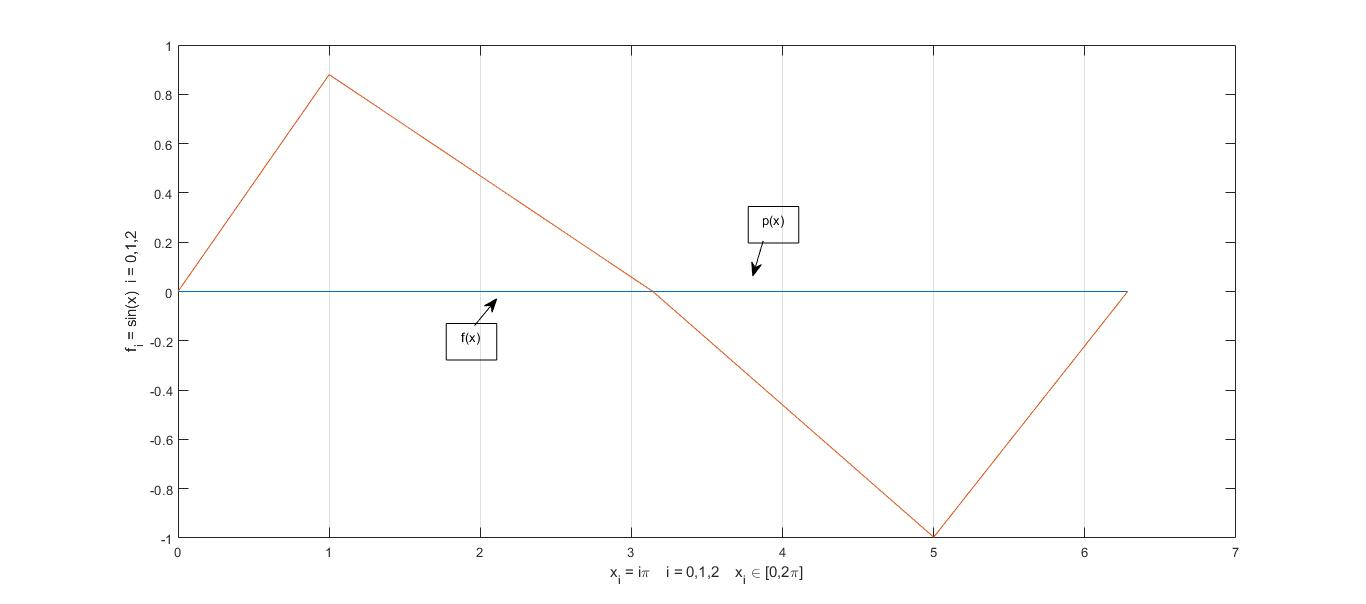
\includegraphics[left, width=150px]{Plot/Cap_4_Es_4_Hermite}
			\caption*{Hermite}
	\end{figure}